\documentclass[review, screen]{acmart}

\acmVolume{0}
\acmNumber{0}
\acmArticle{0}
\acmYear{2019}
\acmMonth{0}

\setcopyright{acmcopyright}

\acmDOI{0000001.0000001}

\bibliographystyle{ACM-Reference-Format}
\citestyle{acmauthoryear}   

\usepackage[english]{babel}
\usepackage[utf8x]{inputenc}

\usepackage{caption}
\usepackage{subcaption}

\usepackage{amsfonts} % mathbb
\usepackage{amsthm}   % environment proof
\usepackage{stmaryrd} % semantical brackets

\usepackage{siunitx} 

\usepackage{xcolor}
\usepackage{graphicx}
\graphicspath{{../gfx/}}
%% \usepackage[hidelinks]{hyperref}

\usepackage{glossaries}
\usepackage{csvsimple}

\newif\ifcomments\commentstrue   %% include author discussion
\ifcomments
\newcommand{\yz}[1]{\textcolor{blue}{{[YZ:~#1]}}}
\newcommand{\bcp}[1]{\textcolor{red}{{[BCP:~#1]}}}
\newcommand{\cvl}[1]{\textcolor{green}{{[CVL:~#1]}}}
\else
\newcommand{\yz}[1]{}
\newcommand{\bcp}[1]{}
\newcommand{\cvl}[1]{}
\fi

\makeatletter 
\let\c@table\c@figure
\let\c@lstlisting\c@figure
\let\ftype@table\ftype@figure
\let\ftype@listings\ftype@figure
\makeatother

\newif\ifopinions\opinionsfalse   %% include author discussion

\newcommand{\python}{\texttt{Python 3}}
\newcommand{\gaz}{\si{\kilogram\of{CO_2e}}}
\newcommand{\gazunit}{\si{\kilogram\of{CO_2e~ per~ passenger}}}
\newcommand{\gazunitbis}{\si{\tonne\of{CO_2e}}}

\newcommand{\event}{event} % What's the right term to designate a specific iteration of a conference?
\newcommand{\conf}{conference} 

\newtheorem{obs}{Observation}
\newtheorem{recommend}{Recommendation}

\title{Engaging with Climate Change: grounding in data possible changes for SIGPLAN}

\begin{document}

\title{Towards Sustainable Conferences: An Analysis of SIGPLAN Conference Data}

\author{Cristina V. Lopes}
%\orcid{1234-5678-9012-3456}
\affiliation{%
  \institution{University of California, Irvine}
  \city{Irvine}
  \state{CA}
  \postcode{92697}
  \country{USA}}
\email{lopes@uci.edu}

\author{Benjamin C. Pierce}
\affiliation{%
  \institution{University of Pennsylvania}
  \city{Philadelphia}
  \state{PA}
  \country{USA}}
\email{bcpierce@cis.upenn.edu}

\author{Yannick Zakowski}
\affiliation{%
  \institution{University of Pennsylvania}
  \city{Philadelphia}
  \state{PA}
  \country{USA}}
\email{zakowski@seas.upenn.edu}

\begin{abstract}

In 2017, ACM's Special Interest Group on Programming Languages (SIGPLAN)
formed an ad-hoc committee to study issues related to climate change---in
particular, how SIGPLAN might contribute to the 40\%\bcp{Or 45??} reduction in carbon
emissions by 2030 that the IPCC tells us is needed to maintain warming under
1.5$^{\circ}$C~\cite{IPCCReport}. One important part of this effort has been
to gather data pertaining to SIGPLAN conferences so to gain a better
understanding of their present emissions. This paper explains the data we
gathered and presents some preliminary analysis of this data. Our main
finding is that there is an inherent conflict between SIGPLAN's goal of
geographic inclusiveness and the goal of reducing carbon emissions, and
that, going forward, innovative approaches for how to organize conferences
that are both inclusive and carbon efficient will be needed.

We believe that other research communities can benefit from performing a
similar introspection and drawing their own conclusions from results. To
this end, we also describe the open-source Python scripts we developed to
conduct our analysis.

\end{abstract}

\keywords{Climate change, conferences, carbon footprint, air travel,
  SIGPLAN, ACM} 

\maketitle

\section{Introduction}

Given the existential threat of global warming, it is incumbent on
individuals and organizations to evaluate the carbon emissions
associated with their activities and find ways to reduce them.  For many
academic researchers, these emissions will overwhelmingly come from air
travel, especially to international conferences.

This observation raises a number of questions about how to organize our
professional activities so as to maximize progress while minimizing
emissions.  Should SIGPLAN conference locations be chosen to minimize their
carbon impact? If
so, how? Should we move toward co-locating conferences? Or, on the contrary,
should some conferences be split into regional meetings or held
simultaneously at two sites on different continents?
Should we continue holding some conferences entirely virtually,
post Covid?
% \bcp{This is a
%   good question, of course, but I'm not sure it is addressed at all by the
%   data we have.}
% \yz{My rationale was that all these questions require hard numbers to ponder
%   correctly, which is the object of this paper. None of these questions should
%   really find an answer here, should it?}

To ground discussions about the decisions and compromises that the
scientific community may collectively wish to undertake, at least three
main sorts of data seem useful.
\begin{itemize}
\item The estimated emissions of past conferences.
\item The geographical distribution of participants to conferences.
\item The overlap in participation between various conferences.
\end{itemize}

We outline the results of a preliminary analysis of the past several
years of registration data for four of the main SIGPLAN conferences.  We
hope this effort can serve as a basis both for debates about concrete
measures and for larger and more comprehensive studies.

After briefly describing our dataset in Section~\ref{sec:dataset}, we
present estimates of the individual footprints of each conference in
Section~\ref{sec:footprint}.  In Section~\ref{sec:community}, the core of
our analysis, we derive several statistics about the geographical
distribution of participants and their habits of
cross-participation---across years and across conferences---arguing that
these data are correlated to the footprint.  We then present in
Section~\ref{sec:speculate} a speculative experiment aiming to estimate
``ideal locations'' for past conferences in order to minimize their
footprints.  \ifopinions In Section~\ref{sec:opinions} we draw some concrete
recommendations for future conference organizers based on these analyses.
\fi Finally, in Section~\ref{sec:software}, we outline the open-source tool
we developed to conduct our analyses, in hopes that other communities might
piggyback on our efforts to conduct their own similar studies.

\section{Dataset}
\label{sec:dataset}
 
Our dataset consists of 10 years worth of attendance to the four major
SIGPLAN conference series---POPL, PLDI, ICFP, and SPLASH---from the
beginning of 2009 until the end of 2018. Data for some of the conferences in the
earlier years are missing. In total, we have data for 33 conferences,
corresponding to 8,758 unique participants and 16,374 trips. For each
participant, we know all the conferences (s)he attended, and from which city
(s)he departed to attend the conferences.
%
The names of participants are replaced in the dataset by unique hashes,
obscuring each individual's identity while allowing them to be identified
across years and across the conferences they attended.



\section{The footprint of conferences: an estimation}
\label{sec:footprint}

Carbon footprint is the essential metric of interest that we seek to reduce.
As such, it is also the starting point of our analysis.
We introduce in this section the methodology we used and tool we built to
conduct all of our analyses, and describe the first results ran on our dataset.

\subsection{Evaluation of the carbon cost: methodology}
\label{sec:methodo}

We conduct all our analyses through a \python{} script, publicly available at
\url{https://github.com/YaZko/acm-climate}. We describe its behavior and give
a brief overview of its use in Section~\ref{sec:software}.
\bcp{Maybe this repo needs a more
informative name?}

For the carbon footprint estimate we present in this paper,
it is relevant to keep in mind the following assumptions that have
been made:
\begin{itemize}
\item we assume that \emph{all} participant travelled by plane;
\item we assume that the airports used are close enough to the end points for their locations to be assimilated;
\item we assume that all flights are direct flights;
\item we assume that the geodesic distance is the one taken by planes.
\end{itemize}

Estimating the errors introduced by these hypotheses and refining them would be
a valuable work. However, for this first proposal that mainly aims at a relative
evaluation of different structural changes in our activities, we believe those
to be workable hypotheses.

The distance traveled by the participants is converted to an emission expressed
in \gaz. To do so, we use a standard model introduced as part of the
\texttt{DEFRA 16} report on Greenhouse gas
\footnote{\url{https://www.gov.uk/government/publications/greenhouse-gas-reporting-conversion-factors-2016}}
\footnote{\url{https://co2calculator.acm.org/methodology.pdf}}
conducted by the British Government.

The model distinguishes three classes of flight, depending on their length:
short, medium or long hauls. Each category is associated with a linear
coefficient relating directly the distance of travel to the amount of \gaz
emitted. We make the assumptions, anecdotally observed, that researchers all
fly in economy class.

A second linear coefficient, identical for all flights and so-called
\emph{radiative forcing index}, is added to account for the difference in
radiative forcing between the same emissions at ground level compared to high in
the atmosphere. This coefficient has been taken for the results presented in this
paper to be $1.891$ as suggested by R. Sausen et al.~\cite{Sausen05}

We therefore obtain the following piece-wise linear model of emissions for a flight covering $d$ kms:
\begin{itemize}
\item $1.891 * 0.14735 * d$ \gazunit if $d < 785$
\item $1.891 * 0.08728 * d$ \gazunit if $785 \leq d < 3700$
\item $1.891 * 0.077610 * d$ \gazunit if $3700\leq d  $
\end{itemize}

%% It should be noted that experiments with other models show significant variance
%% in absolute value, but resilience in relative values.\bcp{Maybe worth
%%   showing some numbers justifying these statements?}\yz{I agree, will
%%   do}\bcp{Assuming that we can get our numbers to agree with CoolEffect's,
%%   we could also mention this!} Once again, refining the
%% model would hence be a valuable work, but using this simple standard and
%% well-established one appears appropriate to draw conclusion in terms of
%% \emph{relative} impact of different measures.

%% This first pass of the script therefore give us an estimation of the footprint
%% of our conferences. We have implemented on top of it several analyses aiming to
%% estimate the correlation some concrete factors upon which conference organizers
%% can act may have with this footprint.
%% The description of these analyses will cover Section~\ref{sec:community} to \ref{sec:speculate}.

\subsection{Footprint of the studied conferences}

\begin{table}
\begin{tabular}{|l|l|c|c|c|}
  \hline%
  \bfseries Event & \bfseries Location & \bfseries \# Participants & \bfseries Total cost & \bfseries Average cost 
\csvreader[head to column names]{../../output/sigplan/footprint_confs.csv}{}%
{\\\conf\ \year & \location & \csvcoliv & \csvcolv & \csvcolvi}%
\\\hline
\end{tabular}
\caption{For each \event: location, number of participants and carbon cost, total and average per participant, in \gazunitbis,}
\label{table:footprint}
\end{table}

We now turn to the estimation of the footprint of our dataset.
Table~\ref{table:footprint} depicts the total and average carbon cost per participant of
all conferences analyzed. This cost is estimated in terms of \gazunitbis of emissions.
The main data of interest is arguably the last column depicting the average cost per participant.

This high level data already suggests an interesting observation:
\begin{obs}
If the carbon footprint of conferences due to air travel is indeed significant,
its specific average value per participant varies from an \event to another by up
to a factor of 2.
\label{obs:footprint}
\end{obs}

Indeed, the lowest average carbon cost of our dataset is obtained by PLDI'18 at 0.9\gazunitbis,
while the highest one is reached by ICFP'16 at 1.93\gazunitbis.
Understanding the underlying rationals for such variations may be a promising
angle to reduce our emissions without restructuring fundamentally our activity.

\section{Data Analysis: Community}
\label{sec:community}

The greenhouse gas emissions from a given \event is in direct proportion to
the average distance traveled by the participants of this \event.
To understand emissions, we must therefore estimate the nature of the
communities that attend each conference.

The aggregated information we describe below falls into two main categories:
first, the demographic distribution of the participants to the conferences
conditioned by various factors, and second, the participation habits of the
community through recurring participation to a given conference and the
overlap in participation between different conferences.

%% Through this section, we present the results of our data analysis in a
%% neutral way. We point out phenomena that came out as a
%% surprise to us, but defer opinionated observations and practical conclusions to
%% Section~\ref{sec:opinions}.

\subsection{Demographics: Where Did Participants Come From?}
\label{subsec:demo}

\begin{figure}
  \centering
  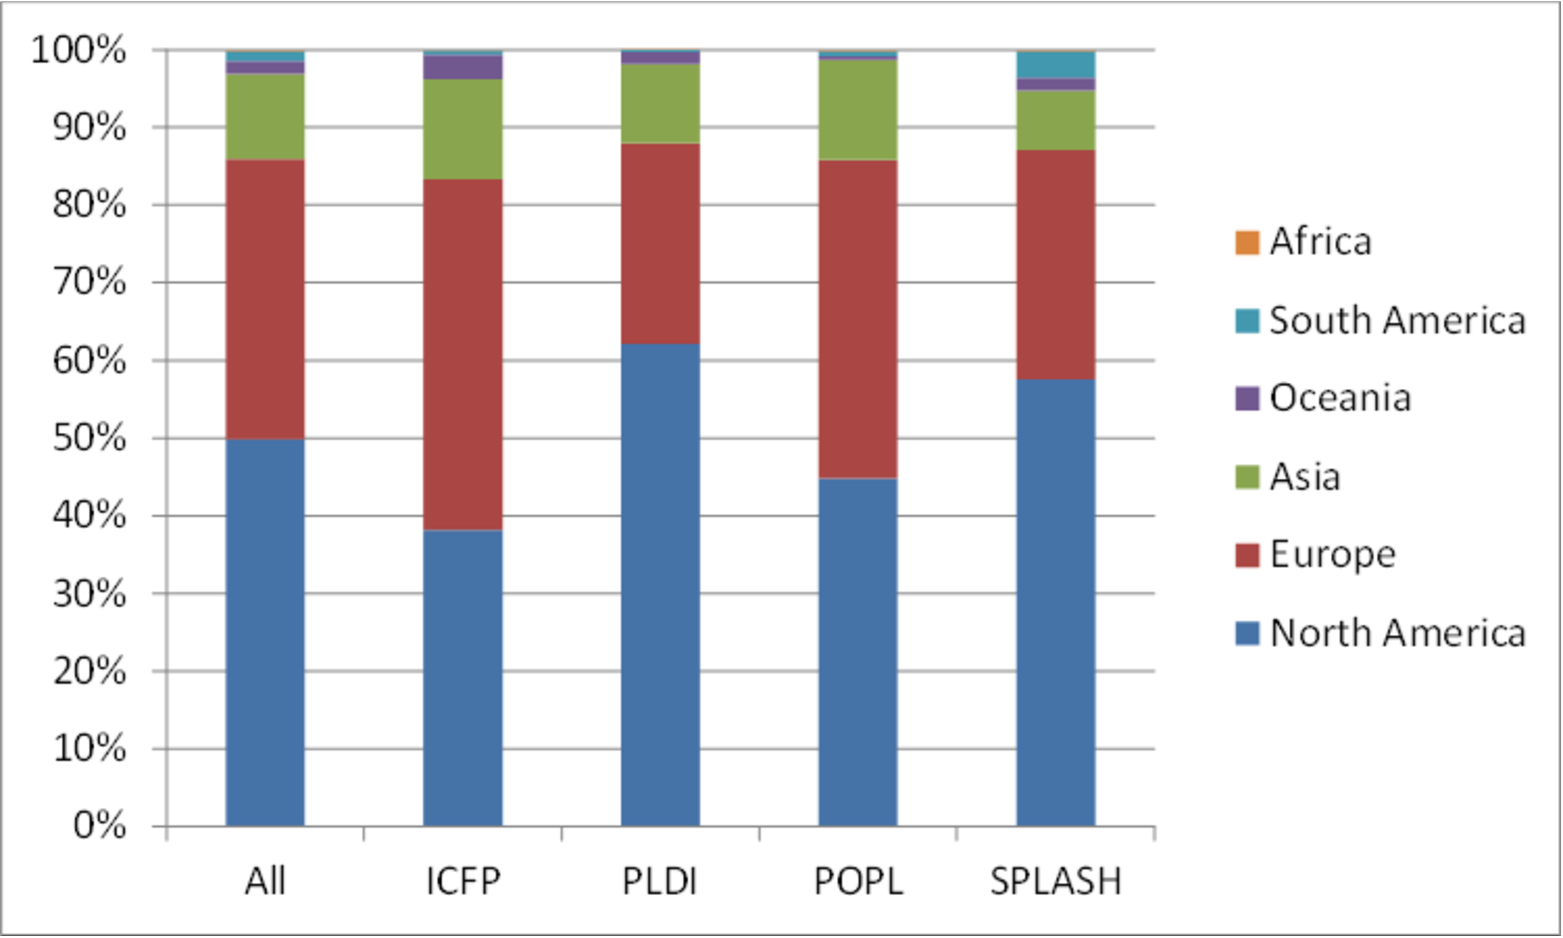
\includegraphics[width=0.7\textwidth]{ParticipantsOrigin.pdf}
  \caption{Overall origin of participants per conference.}
  \label{fig:demo-per-conf}
\end{figure}

\begin{table}
    \centering
    \csvreader[%
      head to column names,
      tabular={|c|c|c|c|c|c|c||c|},
      table head=\hline \bfseries Conference & \bfseries EU (\%) & \bfseries NA (\%) & \bfseries AS (\%) & \bfseries SA (\%) & \bfseries AF (\%) & \bfseries OC (\%) & \bfseries Local (\%)\\\hline,
      table foot = \hline,
      late after line=\ifthenelse{\equal{\Conference}{Any}}{\\\hline}{\\},
    ]{../../output/sigplan/demographic_per_conf.csv}{}{%
      \Conference & \EU & \NA & \AS & \SA & \AF & \OC & \Local \
    }

   \caption{For each kind of conference, distribution of participants per continent of origin.
     Among all participants of a category of conferences, displays the percentage of these participants that traveled from the indicated continent. The \textbf{Local} column uses for each instance of the conference the same continent as the one the conference took place in. The line \emph{Any} computes the same data, but across all conferences at once.
   }
\label{table:demo-per-conf}
\end{table}


Figure~\ref{fig:demo-per-conf}\footnote{The graphical representations in
  this preliminary draft are based on a slightly different version of our
  dataset than the one used by our tool. There may be some minor
  discrepancies between these representations and the raw tables
  presented.\bcp{Hopefully we can remove this!  Or, if it's just the big
    red-and-green table, we can at least move this comment there.}} and Table~\ref{table:demo-per-conf} show
where all participants came from, grouped by ``continents'': North and South
America, Europe, Asia, Africa, and Oceania. For each conference, we depict the
distribution of attendance per continent. Table~\ref{table:demo-per-conf}
shows the portion of attendants originating from the same continent as the
one the event took place in. To a first approximation, maximizing this last
metric, i.e. hosting conferences in the continent containing the majority of
its community, is a good thing.

Taken as a whole, these conferences attracted 50\% of their participants
from North
America, 36\% from Europe, 11\% from Asia, 2\% from Oceania, 1\% from South
America, and less than 0.2\% from Africa.
The data also shows some degree of geographical affinity for the
various conferences:
PLDI and SPLASH appear to be quite North-America-centric, while
ICFP's core community has a strong anchor in Europe as well.

\begin{table}
  \centering
  \csvreader[%
    head to column names,
    tabular={|c|c||c|c|c|c|c|c||c|},
    table head=\hline \bfseries Event & \bfseries Location & \bfseries EU (\%) & \bfseries NA (\%) & \bfseries AS (\%) & \bfseries SA (\%) & \bfseries AF (\%) & \bfseries OC (\%) & \bfseries Local (\%)\\\hline,
    table foot = \hline,
    late after line=\\,
  ]{../../output/sigplan/demographic.csv}{}{%
    \Conference~\Year & \Continent & \EU & \NA & \AS & \SA & \AF & \OC & \Local \
  }
  \caption{For each \event, the continent in which it took place and
    the distribution of attendance per continent of origin of participants.
    The final column indicates the
    portion of participants that did not change continent to attend the conference.}
  \label{table:demo-per-event}
\end{table}

\begin{figure}
  \centering
  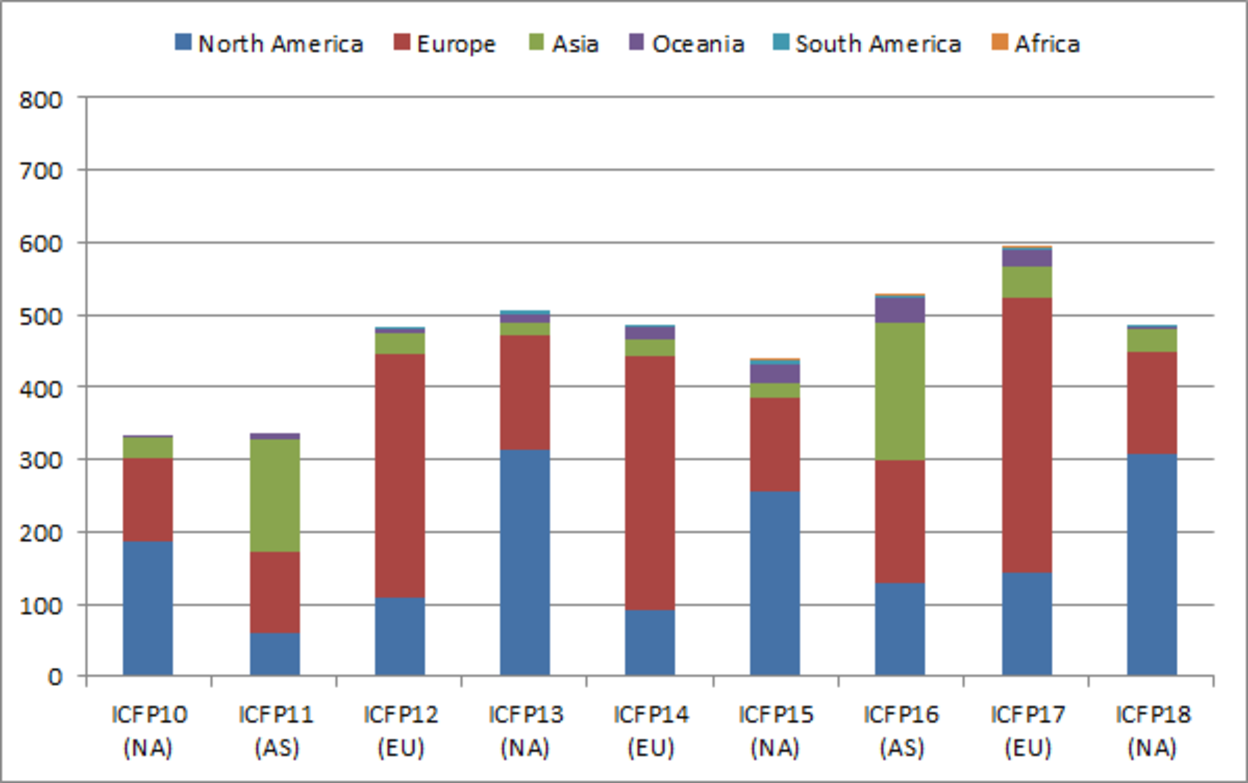
\includegraphics[width=0.45\textwidth,height=1.8in]{ParticipantsOriginICFP.pdf}
  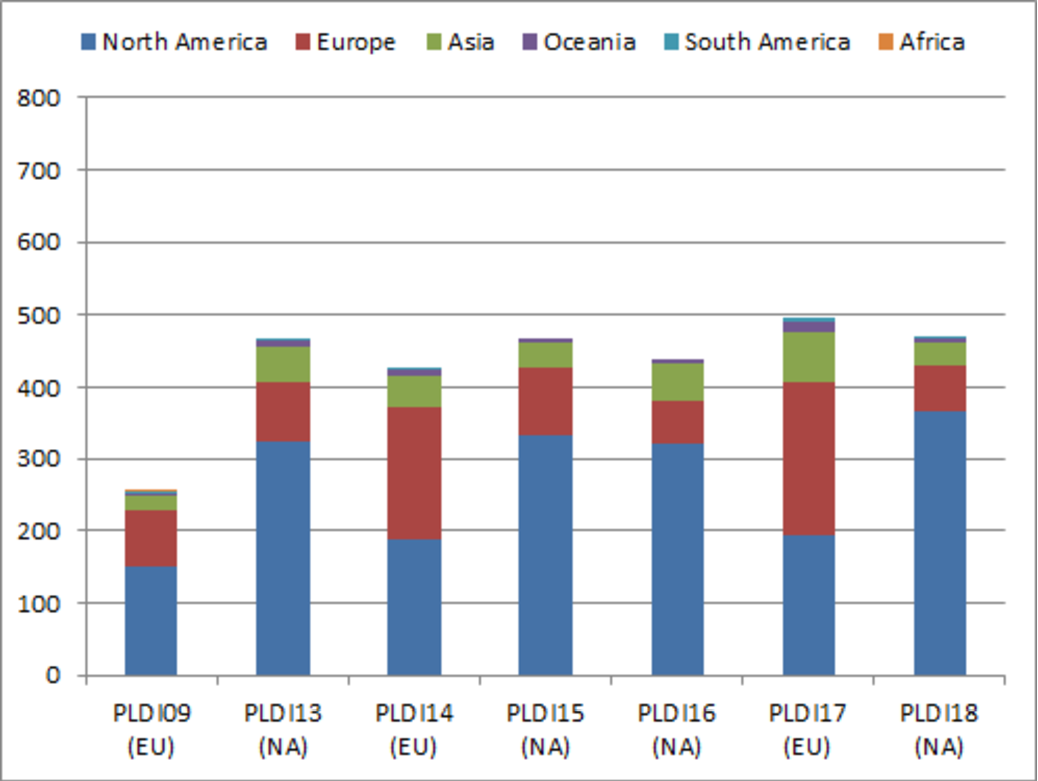
\includegraphics[width=0.45\textwidth,height=1.8in]{ParticipantsOriginPLDI.pdf}
  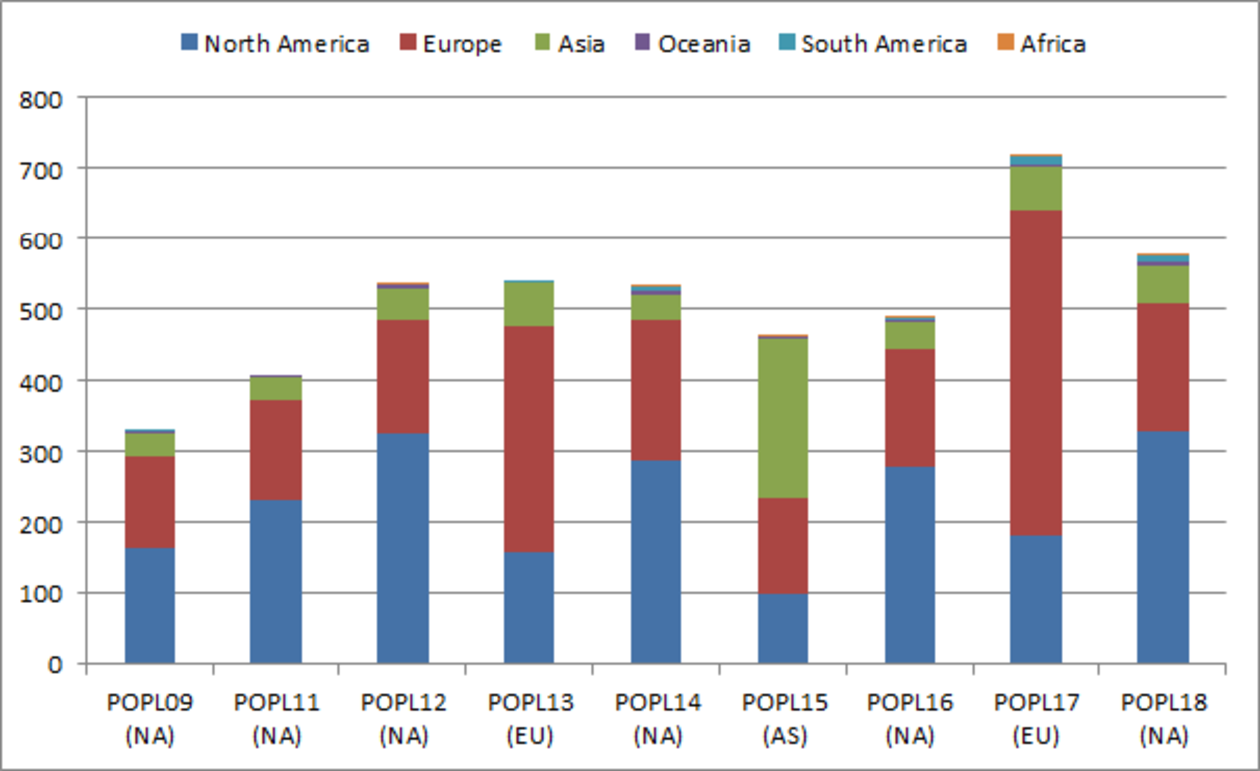
\includegraphics[width=0.45\textwidth,height=1.8in]{ParticipantsOriginPOPL.pdf}
  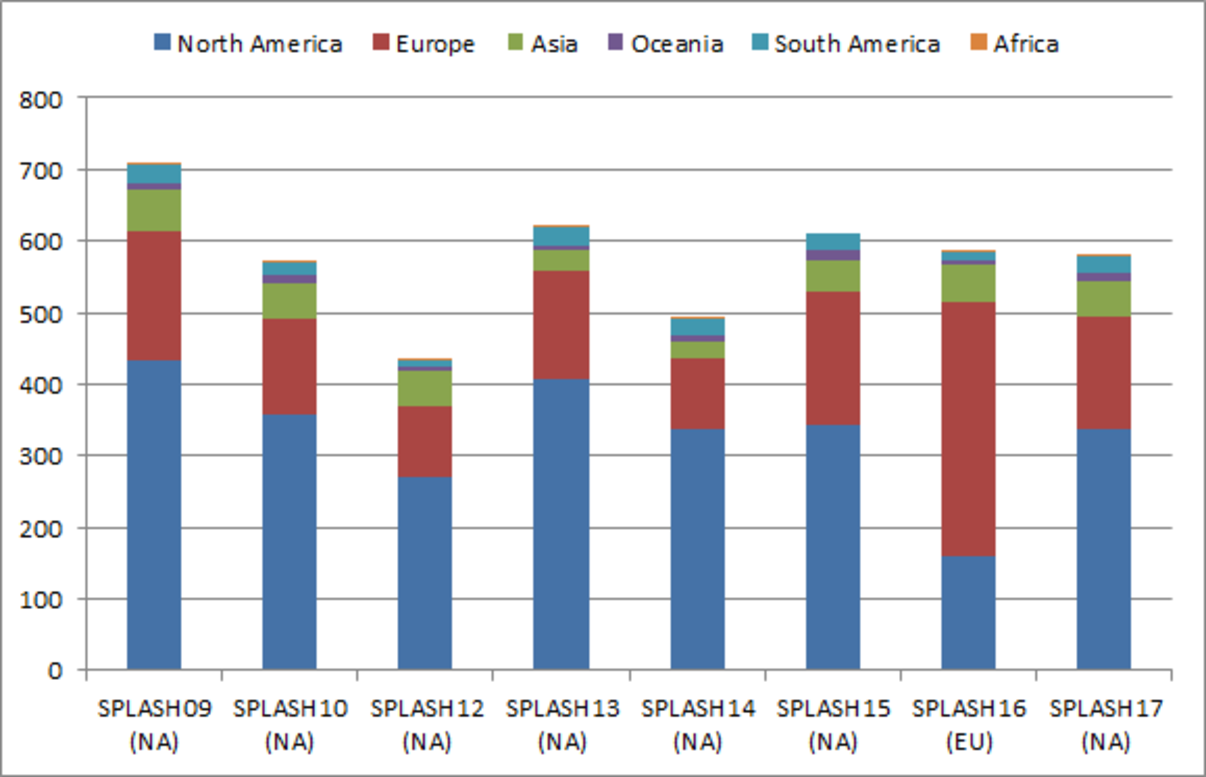
\includegraphics[width=0.45\textwidth,height=1.8in]{ParticipantsOriginSPLASH.pdf}
  \caption{Origin of participants for each conference, detail.}
  \label{fig:demo-per-event}
\end{figure}

This overall picture, however, hides some interesting facts pertaining to the
relationship between the conferences' locations and the origin of the participants.
Indeed, aggregating the attendance per conference intrinsically rests upon the
assumption of a uniform community that attends every instance of the conference
every year.  This picture turns out to be quite misleading.

Table~\ref{table:demo-per-event} and Figure~\ref{fig:demo-per-event}
show a more detailed breakdown of the origin of participants for each
conference, showing also the geographic region where the conferences were held.
%
These charts make it clear that the location of the conference had a
substantial effect on the distribution of attendees, with each conference
tending to attract people from the same geographic area. This
effect is quite visible for ICFP and POPL, with noticeable ups and downs of
the colored bars between North American and European participants when the
conferences were located in North America and Europe, respectively. Most
strikingly, Asian participation during POPL '15, ICFP '11 and ICFP '16,
events that took place on the Asian continent, is significantly higher than
the rest: there appears to be a strong locality phenomenon
here. Cross-referencing this data
with Table~\ref{table:footprint}, one can also notice that the only time
SPLASH took place in Europe also turned out to be the least carbon-intensive
edition, challenging the previous observation, based on a high-level view
of past attendance data, that the conference might appear to
be mostly North-America-centric.

\begin{table}
  \centering
  \csvreader[%
    head to column names,
    tabular={|c||c|c|c|c|c|c||c|},
    table head=\hline \bfseries Location & \bfseries EU (\%) & \bfseries NA (\%) & \bfseries AS (\%) & \bfseries SA (\%) & \bfseries AF (\%) & \bfseries OC (\%) & \bfseries Local (\%)\\\hline,
    table foot = \hline,
    late after line=\ifthenelse{\equal{\Location}{Any}}{\\\hline}{\\},
  ]{../../output/sigplan/demographic_delta.csv}{}{%
     \Location & \EU & \NA & \AS & \SA & \AF & \OC & \Local 
  }
  \caption{Geographical distribution of participation conditioned by the
    location of the \event: each row indicates the continent in which the
    conference took place, and each cell of this row depicts the percentage of
    participants of these conferences that originated from a given continent.
    The column \textbf{Local} corresponds to the same continent as the conference.}
\label{table:local_effect}
\end{table}

Table~\ref{table:local_effect} attempts to measure this locality effect. The
table depicts, all conferences being considered at once, the geographical
distribution of attendance conditioned by the geographical location of the
\event. The Asian phenomenon previously hinted at is here extremely
apparent: while overall, on average, 10.9\% of the participants come from Asia,
this number is roughly multiplied by a factor 4 when the \event takes place
in Asia (without any significant drop in total volume of attendance that
could indirectly bump this percentage).
Interestingly, this phenomenon also exists in the case of Europe (+22.29\%
deviation from the average) and North America (+12.15\% deviation from the
average).
Thus, despite their name, individual instances of international conferences
appear to exhibit a fairly strong local component.

Overall, this data shows that the goal of increasing geographic inclusion was,
indeed, accomplished by organizing the conferences in diverse parts
of the world. It also places Figure~\ref{fig:demo-per-event} in a broader
context:
a naive interpretation of that chart might lead us to conclude that North
America and Europe are where most of this community is, but it is not that
simple. Because of the regional effect on participation, the distribution of
participants also reflects the fact that most of these conferences were {\em
  held} in
North America and Europe (30), only a few were held in Asia (3), and none in
South America, Oceania, or Africa.

The situation may be summed up in two elementary observations:
\begin{obs}
  The vast majority of participants are split between North America and
  Europe, with the remainder mostly coming from
  Asia. SPLASH and PLDI are strongly anchored in North
  America. ICFP and POPL fairly equally split between North America and Europe.
  \label{obs:dist-naive}
\end{obs}
This distribution, however, is \emph{strongly} dependent on the
location of the \event.
\begin{obs}
  There is also a strong locality effect in conference attendance: nearby
  conferences attract significant numbers of new participants from the area,
  while longer distances discourage some participants.
  \label{obs:locality}
\end{obs}

\subsection{How Often Did Participants Attend These Conferences?}
\label{subsec:overlap}

Section~\ref{subsec:demo}, through the study of the demographic distribution of
attendance, has suggested the existence of local communities that only
partake in conferences when they take place close to their place of residency.
One can conversely look for groups of ``regular attendees'' that participate in
a given \conf regardless of where it is held.

\begin{figure}
  \centering
  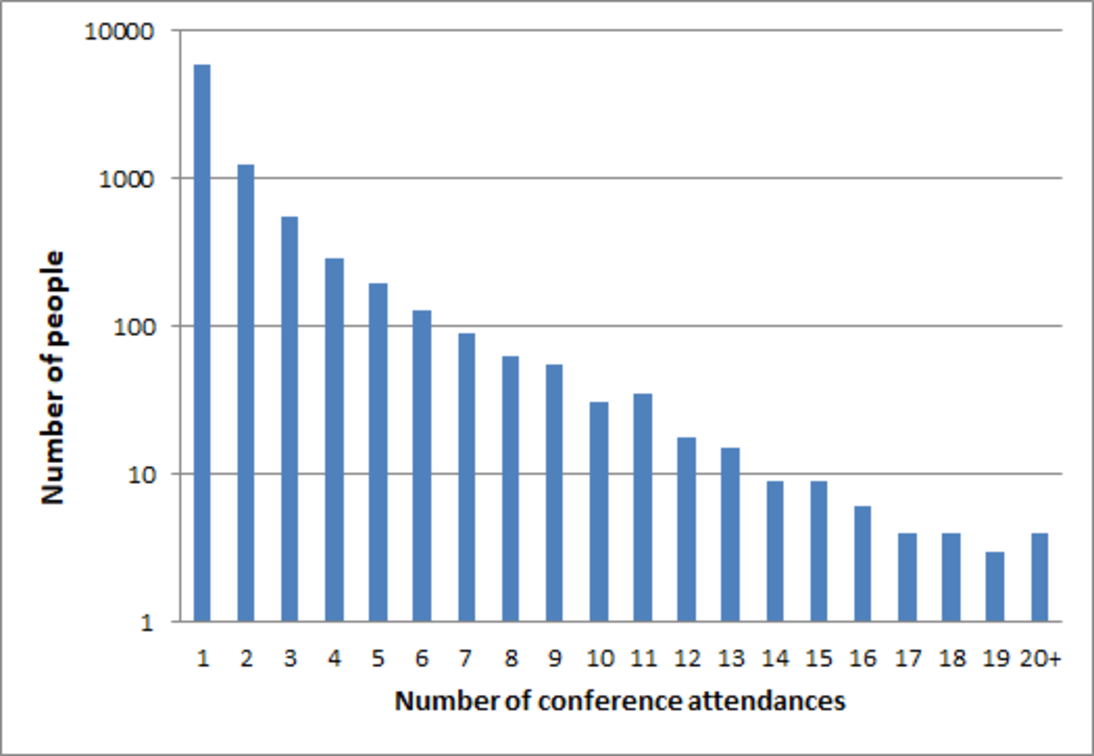
\includegraphics[width=0.6\textwidth]{AttendanceHist.pdf}
  \caption{Histogram of attendance.}
  \label{fig:hist_attendance}
\end{figure}

\begin{figure}
  \centering
  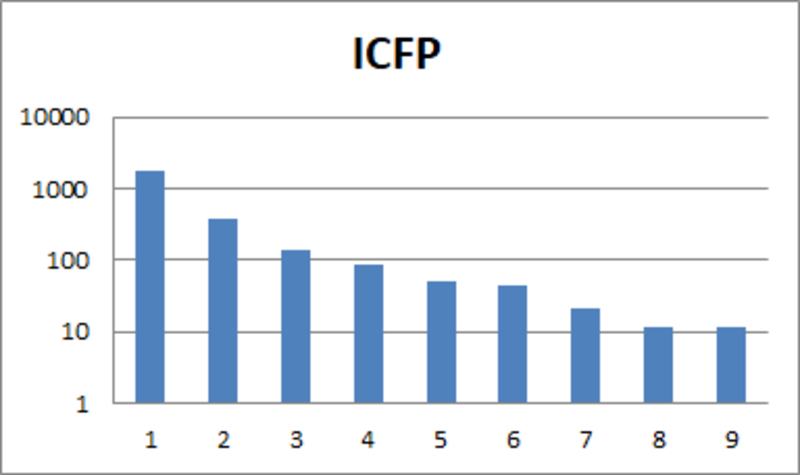
\includegraphics[width=0.45\textwidth,height=1.5in]{AttendanceHistICFP.pdf}
  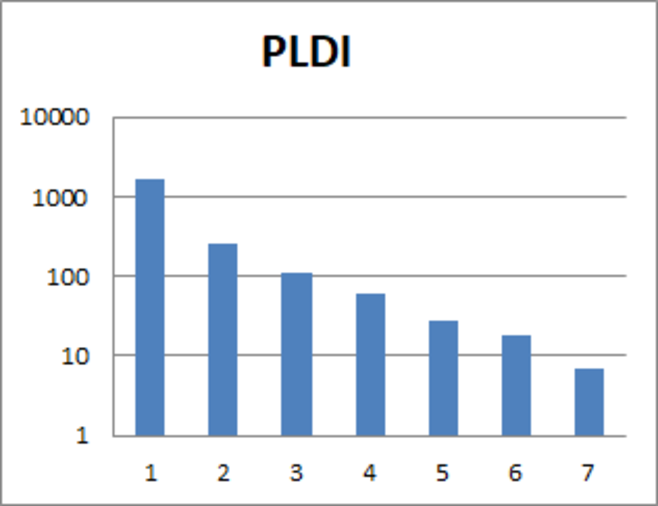
\includegraphics[width=0.4\textwidth,height=1.5in]{AttendanceHistPLDI.pdf}
  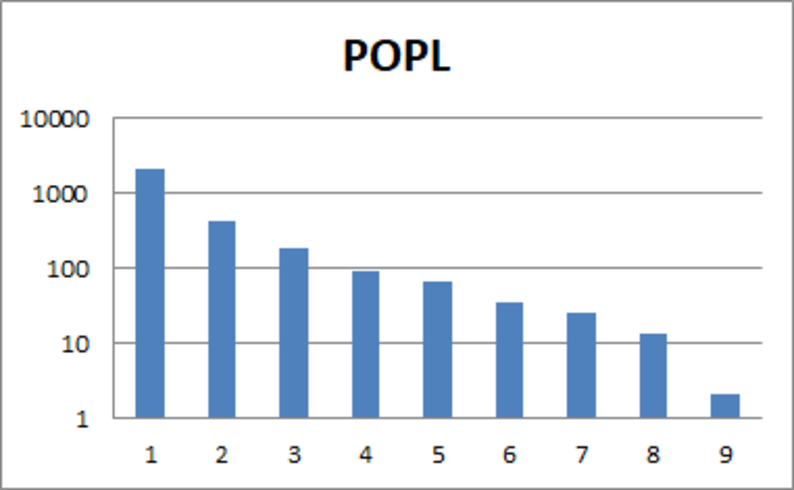
\includegraphics[width=0.45\textwidth,height=1.5in]{AttendanceHistPOPL.pdf}
  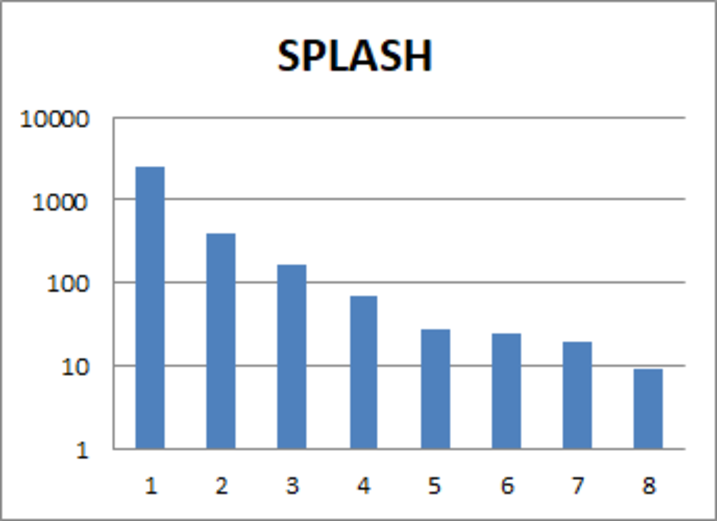
\includegraphics[width=0.4\textwidth,height=1.5in]{AttendanceHistSPLASH.pdf}
  \caption{Histogram of attendance for each conference series.}
  \label{fig:hist_attendance_per_conference}
\end{figure}

Figure~\ref{fig:hist_attendance} shows how often the same participants attended
multiple conferences. At the extremes, 6,009 people (69\%) attended only 1
conference, and just 4 people attended 20 or more conferences. Participation is
dominated by single-conference participants, perhaps reflecting a large and
transient student population. The pattern is similar for each conference series,
shown in Figure~\ref{fig:hist_attendance_per_conference}.


\subsection{What Was the Participation Overlap Between These Conferences?}

We now take a closer look at the habits of these recurring participants.

\begin{table}
  \centering
  \begin{subtable}[!t]{0.48\textwidth}
    \centering
    \csvreader[%
      head to column names,
      tabular={|c|c|c|c|},
      table head=\hline \bfseries Year & \bfseries Overlap & \bfseries \#ICFP & \bfseries \#POPL \\\hline,
      table foot = \hline,
      late after line=\ifthenelse{\equal{\Year}{All}}{\\\hline}{\\},
    ]{../../output/sigplan/overlap_cross_conf_ICFP_POPL.csv}{}{%
      \Year & \Overlap & \csvcoliii & \csvcoliv
    }
    \caption{ICFP and POPL}
  \end{subtable}
  \hspace{\fill}
  \begin{subtable}[!t]{0.48\textwidth}
    \centering
    %% \flushright
    \csvreader[%
      head to column names,
      tabular={|c|c|c|c|},
      table head=\hline \bfseries Year & \bfseries Overlap & \bfseries \#POPL & \bfseries \#PLDI \\\hline,
      table foot = \hline,
      late after line=\ifthenelse{\equal{\Year}{All}}{\\\hline}{\\},
    ]{../../output/sigplan/overlap_cross_conf_POPL_PLDI.csv}{}{%
      \Year & \Overlap & \csvcoliii & \csvcoliv
    }
    \caption{POPL and PLDI}
  \end{subtable}
  \newline
  \vspace*{0.1cm}
  \newline

  \begin{subtable}[!t]{0.48\textwidth}
    \centering
    \csvreader[%
      head to column names,
      tabular={|c|c|c|c|},
      table head=\hline \bfseries Year & \bfseries Overlap & \bfseries \#POPL & \bfseries \#SPLASH \\\hline,
      table foot = \hline,
      late after line=\ifthenelse{\equal{\Year}{All}}{\\\hline}{\\},
    ]{../../output/sigplan/overlap_cross_conf_POPL_SPLASH.csv}{}{%
      \Year & \Overlap & \csvcoliii & \csvcoliv
    } 
    \caption{POPL and SPLASH}
  \end{subtable}
  \hspace{\fill}
  \begin{subtable}[!t]{0.48\textwidth}
    \centering
    %% \flushright
    \csvreader[%
      head to column names,
      tabular={|c|c|c|c|},
      table head=\hline \bfseries Year & \bfseries Overlap & \bfseries \#ICFP & \bfseries \#PLDI \\\hline,
      table foot = \hline,
      late after line=\ifthenelse{\equal{\Year}{All}}{\\\hline}{\\},
    ]{../../output/sigplan/overlap_cross_conf_ICFP_PLDI.csv}{}{%
      \Year & \Overlap & \csvcoliii & \csvcoliv
    }
    \caption{ICFP and PLDI}
  \end{subtable}
  \newline
  \vspace*{0.1cm}
  \newline

  \begin{subtable}[!t]{0.48\textwidth}
    \centering
    \csvreader[%
      head to column names,
      tabular={|c|c|c|c|},
      table head=\hline \bfseries Year & \bfseries Overlap & \bfseries \#ICFP & \bfseries \#SPLASH \\\hline,
      table foot = \hline,
      late after line=\ifthenelse{\equal{\Year}{All}}{\\\hline}{\\},
    ]{../../output/sigplan/overlap_cross_conf_ICFP_SPLASH.csv}{}{%
      \Year & \Overlap & \csvcoliii & \csvcoliv
    }
    \caption{ICFP and SPLASH}
  \end{subtable}
  \hspace{\fill}
  \begin{subtable}[!t]{0.48\textwidth}
    %% \flushright
    \centering
    \csvreader[%
      head to column names,
      tabular={|c|c|c|c|},
      table head=\hline \bfseries Year & \bfseries Overlap & \bfseries \#PLDI & \bfseries \#SPLASH \\\hline,
      table foot = \hline,
      late after line=\ifthenelse{\equal{\Year}{All}}{\\\hline}{\\},
    ]{../../output/sigplan/overlap_cross_conf_PLDI_SPLASH.csv}{}{%
      \Year & \Overlap & \csvcoliii & \csvcoliv
    }
    \caption{PLDI and SPLASH}
  \end{subtable}
  \caption{For every year, we display the number of participants that attended two given conferences.
    We also indicate the total attendance of each event for reference.
    The \emph{All} row depicts the sum over all years.}
  \label{table:overlap-cross}
\end{table}

A first natural question is whether there is significant overlap
in participation between conferences.
Table~\ref{table:overlap-cross} depicts, for each pairing of the four
conferences, the percentage of overlap. This measure is strikingly
low for most conferences.

\begin{obs}
Cross-conference overlap is low: the tightest pairing sees slightly over
10\% of common attendance for a given year. Extending the overlap among any
two years, the tightest pairing still sees less than a quarter of unique
participants having participated at least once in both conferences.
\bcp{This may be the observation that people will be most interested in.  Is
  there any more we can say about it?  Are the statistics we're presenting
  really the most revealing ones?  Also: The figure is presented in abvolute
  nunbers, while the tables use
  percentages.  Maybe we should stick with one or the other? }
  \label{obs:overlap-cross}
\end{obs}

%% \begin{table}
%% \centering
%%      \begin{subtable}[b]{0.4\textwidth}
%%        \centering
%%        \csvautotabular{../../output/sigplan/overlap_intra_conf_POPL.csv}
%%        \caption{Case of POPL}
%%      \end{subtable}
%%      \hfill
%%      \begin{subtable}[b]{0.4\textwidth}
%%        \centering
%%        \csvautotabular{../../output/sigplan/overlap_intra_conf_ICFP.csv}
%%        \caption{Case of ICFP}
%%     \end{subtable}

%%      \caption{For any two years, percentage of overlap in attendance at the corresponding editions of a conference (part 1)}
%%      \label{table:overlap-conf-alpha}
%% \end{table}

%% \begin{table}
%% \centering
%%      \begin{subtable}[b]{0.4\textwidth}
%%        \centering
%%        \csvautotabular{../../output/sigplan/overlap_intra_conf_PLDI.csv}
%%        \caption{Case of PLDI}
%%      \end{subtable}
%%      \begin{subtable}[b]{0.4\textwidth}
%%        \centering
%%        \csvautotabular{../../output/sigplan/overlap_intra_conf_SPLASH.csv}
%%        \caption{Case of SPLASH}
%%      \end{subtable}

%%      \caption{For any two years, percentage of overlap in attendance at the corresponding editions of a conference (part 2)}
%%      \label{table:overlap-conf-beta}
%% \end{table}

\begin{figure}
  \centering
  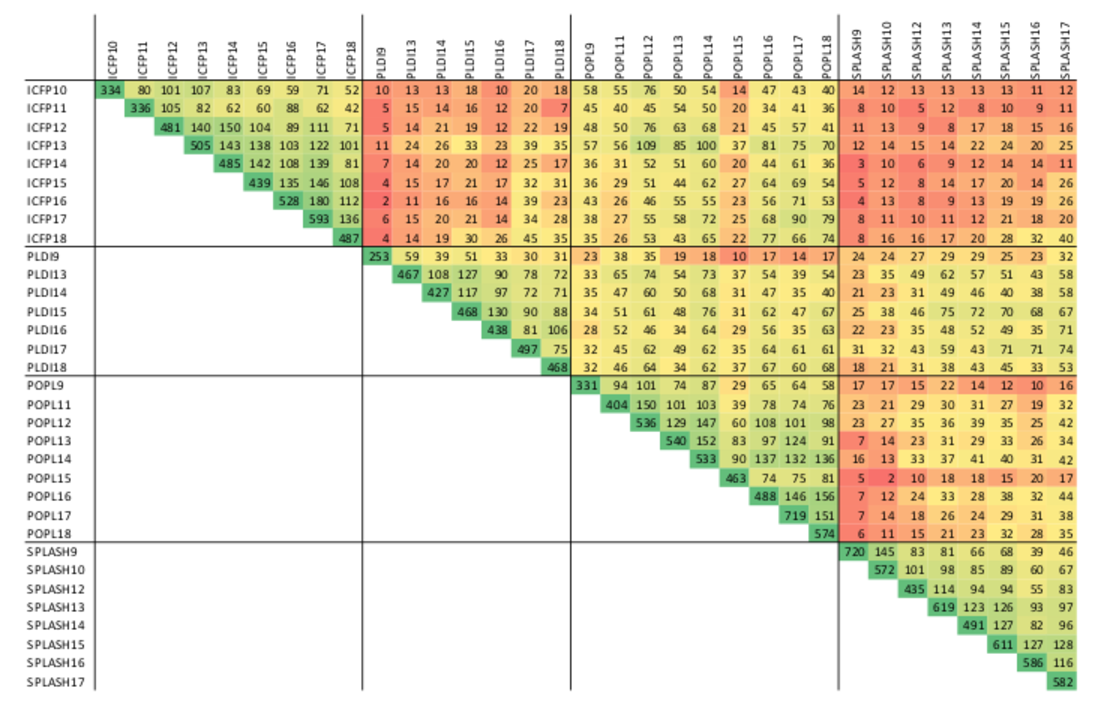
\includegraphics[width=\textwidth]{OverlapAnalysis-crop.pdf}
  \caption{Conference participation overlap.}
  \label{fig:overlap}
\end{figure}

Conversely, one can estimate the overlap for a given conference over time: for a
given conference at a time, and for any pair of years, compute the percentage of
attendees that participated in both events. This new information, as well as
the essential of Table~\ref{table:overlap-cross}, is synthesized graphically on
Figure~\ref{fig:overlap}.
With this bird-eye view of the permanence vs. transience of the
participants over time in SIGPLAN conferences, we can make a second observation,
temporal this time:

\begin{obs}
Temporal overlap is moderate: roughly a quarter of attendees at a given
conference were also present the year before at the same conference.
  \label{obs:overlap-temp}
\end{obs}

In principle, it is desirable to have a balance between repeat participants and
newcomers. Communities that don't attract new participants tend to stagnate; but
communities that don't have a core of repeat participants tend to lose focus.

The existence of a stable community associated with each conference series
(i.e., a group that
tends to repeat participation) is clearly visible near the diagonal in
Figure~\ref{fig:overlap}. The highest overlap of all in particular was between
ICFP'16 and ICFP'17, with 180 repeaters. The four conference series show
what seems to us to be a healthy balance between repeat participation and
newcomers.

The weaker overlap between conferences in different series is also apparent.
The strongest overlap is between PLDI and POPL, followed by ICFP and POPL
and by PLDI and SPLASH. The weakest overlaps are between ICFP and SPLASH,
followed by ICFP and PLDI, and by POPL and SPLASH. It is unclear whether the
overlap, or lack thereof, between these conference series is due to
intellectual reasons or due to their dates. PLDI and POPL is the pair that
is most distant in time, typically June and January. Conversely, ICFP and
SPLASH is the pair that is the closest in time, typically September and
October.  One might conjecture that temporal proximity discourages
cross-participation.

\begin{table}
  \centering
  \csvreader[%
    head to column names,
    tabular={|l|c|c|c|c|c|c|},
    table head=\hline \bfseries Conference & \bfseries Avrg & \bfseries Avrg $\geq$ 2 & \bfseries $\geq$ 2 (\%) & \bfseries $\geq$ 3 (\%) & \bfseries $\geq$ 4 (\%) & \bfseries $\geq$ 5 (\%) \\\hline,
    table foot= \hline,
    late after line=\ifthenelse{\equal{\Conference}{All}}{\\\hline}{\\},
  ]{../../output/sigplan/number_of_participations_per_conf.csv}{}{%
    \Conference & \csvcolii & \csvcoliii & \csvcoliv & \csvcolv & \csvcolvi & \csvcolvii
  }
\caption{For each conference and overall, the average number of instances a
  unique individual has taken part of (\textbf{Avrg}), and the same data without
  considering individual that has participated exactly once (\textbf{Avrg} $\geq$ \textbf{2}).
  The other columns display the percentage of participants that have
  attended at least $k$ instances, for $k\in\llbracket 2 \dots 5
  \rrbracket$. Note that the means and percentages are computed with
  respect to the number of \emph{unique} participants. }
\label{table:recurrent}
\end{table}

\begin{table}
  \centering
  \csvreader[%
    head to column names,
    tabular={|l|c|c|c|c|c|},
    table head=\hline \bfseries Year & \bfseries Avrg & \bfseries Avrg $\geq$ 2 & \bfseries $\geq$ 2 (\%) & \bfseries $\geq$ 3 (\%) & \bfseries $\geq$ 4 (\%) \\\hline,
    table foot= \hline,
    late after line=\ifthenelse{\equal{\Year}{All}}{\\\hline}{\\},
  ]{../../output/sigplan/number_of_participations_per_year.csv}{}{%
    \Year & \csvcolii & \csvcoliii & \csvcoliv & \csvcolv & \csvcolvi 
  }
  \caption{For each year, the average number of conferences a participant has participated
    in among POPL, PLDI, ICFP and SPLASH (\textbf{Avrg}),
    and the same data without considering individual that has participated exactly once (\textbf{Avrg} $\geq$ \textbf{2}).
  The other columns display the percentage of participants that have
  attended at least $k$ conferences, for $k\in\llbracket 2 \dots 4
  \rrbracket$. Note that the means and percentages are computed with
  respect to the number of \emph{unique} participants. }
\label{table:recurrent-year}
\end{table}


\begin{table}
  \centering
  \begin{subtable}[b]{0.4\textwidth}
    \centering
    \csvreader[%
      head to column names,
      tabular={|c|c|},
      table head=\hline \bfseries Year & \bfseries Old timers (\%)  \\\hline,
      table foot= \hline,
      late after line=\\,
    ]{../../output/sigplan/old_timer_POPL.csv}{}{%
      \year & \csvcolii 
    }
    \caption{Case of POPL}
  \end{subtable}
  \begin{subtable}[b]{0.4\textwidth}
    \centering
    \csvreader[%
      head to column names,
      tabular={|c|c|},
      table head=\hline \bfseries Year & \bfseries Old timers (\%)  \\\hline,
      table foot= \hline,
      late after line=\\,
    ]{../../output/sigplan/old_timer_ICFP.csv}{}{%
      \year & \csvcolii 
    }
    \caption{Case of ICFP}
  \end{subtable}
  \begin{subtable}[b]{0.4\textwidth}
    \centering
    \csvreader[%
      head to column names,
      tabular={|c|c|},
      table head=\hline \bfseries Year & \bfseries Old timers (\%)  \\\hline,
      table foot= \hline,
      late after line=\\,
    ]{../../output/sigplan/old_timer_PLDI.csv}{}{%
      \year & \csvcolii 
    }
    \caption{Case of PLDI}
  \end{subtable}
  \begin{subtable}[b]{0.4\textwidth}
    \centering
    \csvreader[%
      head to column names,
      tabular={|c|c|},
      table head=\hline \bfseries Year & \bfseries Old timers (\%)  \\\hline,
      table foot= \hline,
      late after line=\\,
    ]{../../output/sigplan/old_timer_SPLASH.csv}{}{%
      \year & \csvcolii 
    }
    \caption{Case of SPLASH}
  \end{subtable}
  \caption{For each conference, percentage of participants that have been
    part of a previous edition of the same conference.}
  \label{table:old-timers}
\end{table}

Finally, Table~\ref{table:recurrent} and \ref{table:old-timers} offer two
different views on recurrent participation. Table~\ref{table:recurrent}
represents respectively for the whole dataset (row ``ALL'') and for each
conference individually the average number of editions a participant has
been part of, as well as the percentage of participants that have been part
of at least a given number of editions of a conference. One striking fact is
that no less than 75\% of unique participants have been to just a single
edition.

Table~\ref{table:old-timers} is a normalization of the information represented
in Figure~\ref{fig:hist_attendance_per_conference}: for each instance of each
conference, it depicts the percentage of participants that have been part of a
previous instance of the conference (in our dataset). Since we take as origin of
time the first year for which we have data, the table is naturally overall monotonic
as years progress. Exceptions can be noticed, such as POPL'15, that seem to indicate
a (proportional) lack of ``old timers''. 

\begin{obs}
Over all conferences, the average number of conferences a given participant
has attended is just 1.52. Less than 4\% of unique participants have been to
more than five events among our dataset.  Similarly, at any given \event,
more than half of the participants were experiencing this conference for the
first time.
\label{obs:old-timers}
\end{obs}


\bcp{General question about all the pictures and tables: Are they
  consistent? (I.e., were the pictures generated from the data in the
  tables, or from earlier versions of that data?)}
\yz{Unfortunately no not at the moment: all tables are generated, but the
  Figures have been manually produced by Crista from her original take on
  the dataset. It would be great to regenerate them from the generated csv
  files, but I do not know how they have been generated exactly.}

%% \section{Data Analysis: Locations}

%% \subsection{How Carbon Efficient Were These Conferences?}

%% Present the results using a couple of metrics

%% \subsection{How Did the Conferences Do in Attracting Local Participants?}

%% Show 1st quartile and median distances

%% \subsection{Were There Geographic Differences Between the Four Conferences?}

%% POPL/ICFP (Europe-centered) vs PLDI/SPLASH (NA-centered)

%% \subsection{What Would Have Been the Ideal Locations for Each Conference?}

\section{A Retrospective Speculation: Picking the Optimal Destination for Past Conferences}
\label{sec:speculate}
%% \paragraph{A naive, retrospective, optimal choice}

\cvl{Try to do this in Google Earth. Caveat: this is a non-linear system,
  because the participants depend partly on the location... so that needs to
  be accounted for.}\bcp{I think this bit with Google Earth doesn't have to
  be done now?} 

We have observed that the location an \event takes place in significantly
impacts the distribution of origin of its participants. However, setting
this factor aside temporarily to consider what could have been the cheapest
location for past conferences, assuming that the change in location would
cause no change in participants, can be an illuminating exercise.

To this end, we chose a fixed number of locations that we believe to be
representative and spread across the relevant parts of the globe: Paris,
Edinburgh, Boston, Los Angeles, Vancouver, Tokyo, Beijing, and Mumbai. We
then reprocessed the dataset to look for the location in this set that would
have led to the lowest carbon footprint for each event, assuming that it
would not have changed the set of participants.

\begin{table}
    \centering
    \csvreader[%
      head to column names,
      tabular={|l|l|c|c|c|c|},
      table head=\hline \bfseries Event & \bfseries Orig. Loc. & \bfseries Orig. Cost & \bfseries Best Loc. & \bfseries Best Cost & \bfseries Saved \\\hline,
      table foot= \hline,
      late after line=\\,
    ]{../../output/sigplan/optimal_loc.csv}{}{%
      \conf\ \year & \csvcoliii & \csvcoliv & \csvcolv & \csvcolvi & \csvcolvii
    }
  \caption{For each \event, depicts the location, among the following arbitrarily fixed list:
    Paris, Edinburgh, Boston, Philadelphia, Los Angeles, Vancouver, Tokyo, Beijing and Mumbai,
    that would have led to the lowest carbon footprint.
    Starred best locations indicates that they coincide with the original one.
    The final column shows the amount
    of \gazunitbis that it would have saved.\bcp{in what units?} \bcp{Could
      we display 0.0 as blank?}
    \yz{I have a doubt about the code that computes this. If we want to keep it I need to check thoroughly what it does}
  }
  \label{table:optimal}
\end{table}

Figure~\ref{table:optimal} depicts the resulting data: for each \event, the
best location, and the average \gazunitbis{} it would have saved. We observe
that in the majority of the events, the locality effect is strong enough
that the optimal location is on the same continent as the actual
location. However, it is striking to see how often the east coast of the US
turns out to be the cheapest destination. In particular, it appears to be
preferable to the west coast in most cases (in spite of the underlying
locality effect that we are ignoring here\bcp{don't remember what we meant
  by this}).

\begin{obs}
Due to the locality effect, past data can act as a heuristic for a worst
case distribution of attendance with respect to the objective function of
minimizing the carbon footprint. Doing so most notably suggests that the
east coast of the US is generally a lower-carbon location than the west
coast for this group of conferences.
  \label{obs:optim}
\end{obs}

%% \section{What-If Scenarios}

In our report~\cite{climate_report}, we mentioned that another approach to addressing climate issues is to rethink the conference culture that has emerged, organically over many decades, in SIGPLAN (and computer science generally) and consider more radical changes to it. We then list a few alternatives. This section presents a forecast of carbon footprint for three of those alternatives, based on the attendance data we have. \emph{Again, we need to make a lot of assumptions and explain them, because this is not a linear system...}

\subsection{What If: Mega Conferences}

\subsection{What If: Regional Conferences}

\subsection{What If: Multi-Site Conferences}



\ifopinions\section{Opinionated interpretation}
\label{sec:opinions}

The data analysis conducted through Section~\ref{sec:data} has put in evidence
several phenomena that we review here.

\bcp{These observations do not seem all that opinionated.  Maybe move them
  earlier, with the figures they refer to?}

The first one is a straight read of the carbon footprint of conferences. 
\begin{obs}
If as is well known the carbon footprint of
conferences due to air travel is significant, the specific number
varies from an \event to another by up to a factor of 2.
\label{obs:footprint}
\end{obs}

The more specific analysis of demographic data, in Section~\ref{subsec:demo},
gives a sense of the rough origin of participants:

\begin{obs}
  The vast majority of participants are split between North America and Europe,
  Asia to a much lesser degree. SPLASH and PLDI are strongly anchored in North
  America, ICFP and POPL fairly equally split between North America and Europe.
  \label{obs:dist-naive}
\end{obs}

This distribution however turns out to be \emph{strongly} dependent on the
location of the \event.

\begin{obs}
  There is a major ``locality" effect: it is both true that locality attract
  new participants, and distance repels some participants.
  \label{obs:locality}
\end{obs}

The extent of this phenomenon should not be underestimated. The example of the
few conferences having taken place in Asia underlines the size of the community
that we fail to encounter otherwise. Also interesting, the surprisingly cheap
footprint of the only time SPLASH took place in Europe may suggest that the
North American anchor of the conference is not intrinsic, but rather a
self-fulfilling prophecy.

Section~\ref{subsec:overlap} provides insights into the expected ``core" community
that would attend most editions of a given conference by analyzing the overlap
in participations that actually took place.

\begin{obs}
  Temporal overlap is moderate: roughly a quarter of attendants were present
  the year before at the same conference.
  \label{obs:overlap-temp}
\end{obs}

\begin{obs}
  Cross-conference overlap is low: the tightest pairing sees slightly over 10\%
  of common attendance for a given year.  \bcp{More aggregated numbers would
  also be interesting, since I suspect that there are quite a few people
  that only go to one big conference a year, but may alternate between
  (e.g.) POPL and PLDI.}
  \label{obs:overlap-cross}
\end{obs}

Additionally, a significant portion of attendees are ``one timer", or close.

\begin{obs}
  The average amount of conferences a participant has been part of is extremely low: 1.52.
  Less than 4\% of unique participants have been to more than five events
  among our dataset\bcp{Is that an accurate way of saying it?  I thought it
    was ``have been to five instances of the same conference.''  (The other
    number would be interesting too---how many people went to 2,3,4,5
    instances of {\em any} of the conferences?}.
  Similarly, at any \event, more than half of the participants are experiencing this specific
  conference for the first time.
  \label{obs:old-timers}
\end{obs}

Lastly, despite the aforementioned locality effect that tends to narrow the
distribution of attendance around the locality the conference actually takes
place in, a crude search for lowest carbon footprint is highly instructive.

\begin{obs}
  Due to the locality effect, past data can act as a heuristic for a worst case
  distribution of attendance with respect to the objective function of
  minimizing the carbon footprint. Doing so most notably suggests that the East
  Coast should often be preferred to the West Coast.
  \label{obs:optim}
\end{obs}

\subsection{A mandatory estimate of the carbon footprint by the conference organizers}

Despite a modest amount of data at our disposition and the use of a rudimentary suit of
analyses, there is no ambiguity about the relative environmental impact the choice of
location to hold a conference in has. In particular, observation~\ref{obs:dist-naive}
suggests that even setting aside any restructuration of our activities, we can hope for
saving a factor 2 by being more acute when choosing destinations. Furthermore,
observation~\ref{obs:optim} emphasizes that even a naive distribution model already gives
us material to do better, while the more ambitious perspective to model the locality effect
that we discussed through this paper would allow us for even more efficient choices.

In this light, we consider it unacceptable to continue choosing locations of conferences
either blindly, or for its scenic value. We should ponder professional relevancy with
ecological imperative. We hence formulate the following simple recommendation, that shall
have no impact on our professional activity, save for the reduction of some leisuring side
product.

\begin{recommend}
It should be made part of the mandatory process of organization of SIGPLAN
conference to estimate the carbon footprint of the options considered, and
to take the results of this analysis into account to finalize the decision.
\end{recommend}

It shall be emphasized that we do not suggest by this to consider the destination
minimizing the carbon footprint as the systematic right choice. Concerns such as
rotating over different parts of the globe or naturally accounting for availability
of qualified universities to organize should remain of major concern. We merely
assess by this recommendation the need to bring carbon footprint into the constraint
system we seek to optimize.

\subsection{A short term experiment: bi-localized or tri-localized conferences}

A considerate choice of destination to organize conferences can lead to a
non-neglectible reduction of their carbon footprint. However, a reduction of
the scale required to match by 2050 the recommendation from the Accords de Paris
will require more drastic measures. More specifically, we need to reduce the cheer
number of flights our activity induces.

There is no denying that it will have an impact on our activity, some of which will
be negative. It is hence more than ever of importance to take a reasoned approach
allowing us to balance optimization of quantitative measures, such as reducing the
carbon footprint, with qualitative imperative, such as maintaining the ideal of
an international, borderless, scientific research.

Interestingly, this novel requirement leads us to pay attention to data that may also be
relevant to our activity beyond the question of carbon footprint. These should be
taken into consideration as well while seeking a lasting restructuration of our
activity. In particular, it is implicit to assume that conferences have to be
geographically international to gather communities of researchers from all over the
world. However, observation~\ref{obs:locality} challenges strongly this intuition:
despite any claim a conference may have, the very fact that it is hold each year in
a single place on Earth rules out a vast amount of international researchers. It is most
striking with respect to programming language communities from Asia, but seems to be
true for Europeans desiring to partake in SPLASH as well for instance.

This statement is also backed up by evidence against its complement: the idea of a core
group of researchers making the essential of all editions of their favorite conference,
while not completely incorrect, is vastly overestimated. Observations~\ref{obs:old-timers}
most notably makes it very clear.

This analysis leads us to push toward strong considerations for experimenting a more
ambitious way to save carbon: giving up on the uniqueness of location of conferences and
experimenting with bi-localized or tri-localized conferences.

\begin{recommend}
  Some conferences should experiment a bi-localized format. Typically, POPL could for
  instance be held simultaneously held in Boston and Paris. A day would span over 12 hours
  instead of the usual 8. The four hours intersecting would be held simultaneously on
  both sites via visioconference. The eight other hours would be retransmitted live and
  have simple support for questions as is already put in practice.\\
  If the initial experiments go well, we recommend a progressive shift toward this
  format becoming the norm, and consideration for a third site.
\end{recommend}

We argue naturally that this change would be a truly ambitious measure to reduce
significantly the carbon footprint of conferences. But furthermore, we believe that
it would also enhance the international dimension of the conference: following
the locality effect, this would most certainly lead to an increase in participation.

A natural opposition would be to state that it is unreasonably to ask for researchers to
follow twelve hours a day of conferences, and that they would therefore miss part of the
talks. We do not deny this fact, but points out that it is already largely the case,
most conferences having two, if not three tracks in parallel.

Yet, it should not be brushed aside that this would remove some precious
physical interactions between researches from different continents. We
nonetheless argue that making these interactions the systematic default at conferences
is an historical incident. Such a restructuration of our activity would probably
be accompanied by an increase in visit to other laboratories. But that would shift
these interactions from the current situation that put hundreds of researchers in the
same building so that extremely small groups get to meet, to a more sensible ``meeting
by need" organization.

\subsection{A long term need: entirely virtualized conferences}

Bi-localized conferences strike a compromise. On the long run, research, as all
activities, shall however ambition to be entirely carbon-free. This ambitious
goal has already been embraced by some conferences\footnote{https://conference.opensimulator.org/2018/}
and seminars\footnote{https://sites.google.com/site/plustcs/}.

While the currently existing cases are either fairly experimental, or of much more
modest size than a conference such as the ones organized by SIGPLAN, they report
encouraging results. As such, we encourage experiments aiming to develop further
these techniques, and bring the cultural change they entail incrementally among
our community.

\begin{recommend}
  We recommend to conduct experiments toward the development of fully virtual
  conferences as a mean to reach a fully sustainable activity by the horizon 2050
  at the latest.
\end{recommend}

\fi
\section{An Open-Source Tool for Analyzing Conference Footprints}
\label{sec:software}

We hope that the analysis we have conducted for a few SIGPLAN conferences
will offer valuable insights for the organizers of these conferences.
Clearly, though, any observations based on our data cannot be taken as
universal facts: the situation heavily depends notably on the geographical
distribution of the underlying research community and on its cultural habits
of attendance. Moreover, the practical conclusions that it should entail may
diverge from one community to another.  Accordingly, we strongly encourage
similar studies to be performed by other groups.

To help with this, we have released an open-source \python{} script that we
have built to be as parameterizable and reusable as possible. All the
analyses presented in this paper have been generated using this
tool.\footnote{The graphical visualizations have been made separately, the
  script currently only generates tables. Extending it to generate graphical
  takes on these tables would be an interesting feature.} The script can be
found at the following github repository:
\url{https://github.com/YaZko/sigplan-carbon-analysis}.
%
We welcome comments, pull requests, etc., and we would be happy to assist
anyone wishing to use the tool for their own analysis.

Detailed documentation is available in the repository. We give here just a
high-level overview.

The script takes as an input a dataset described by two \texttt{csv}
files. The first one describes the list of conferences: each line describes
a specific event and the location it took place in, i.e. has the fields
\texttt{Name, Year, City, State} and \texttt{Country}. The second one
contains the list of participants of these events: each line describes a
unique participation at an event, with the location of origin of the
participant, i.e., it  has the fields \texttt{Identifier, City, State, Country,
  Conference} and \texttt{Year}.

The first pass of the analysis computes the needed raw data.  Informal named
locations manually provided by participant are mapped to their ISO
designation using the \texttt{pycountry} library.  Once this is done, these
named locations are converted to GPS locations using the \texttt{geopy}
library, which provides a straightforward API to do this.  To avoid
duplicating requests to online APIs, all of these computations are cached
locally.

Distances in kilometers between locations are then computed between GPS
locations once again using the \texttt{geopy} library. They use the geodesic
distance (shortest distance for an ellipsoidal model of the Earth) with a
model providing precision that is several orders more precise than we need.

At this point, we know, for each participant in a conference, the
distance they traveled. The script then uses a model that computes the
carbon footprint of air travel based on this information. For the analysis
presented in this paper, we used the \texttt{DEFRA 16} model described in
Section~\ref{sec:methodo}, but we are also experimenting with a similar one
developed by
\texttt{CoolEffect}.\footnote{\url{https://www.cooleffect.org/}}  As long as
models are functions of the distance, more can be easily added.

This first pass of the script therefore gives us an estimate of the
footprint of our conferences. The analyses described through Section~\ref{sec:community}
are implemented on top of it.
The output of these analyses is encoded into \texttt{csv} tables that can be
used as-is or as the basis of visualization exercises.

There are room for improvement on pretty much all sides---different
footprint models, more complex analyses, and automating the visualization of
the data, to cite just a few. But we hope that this preliminary tool will
form the basis for fruitful discussion as it grows to address the needs of
more research communities.

\section{Conclusion}

We advocate for carbon footprint to be a central constraint driving the logistic
choices made during the organization of a conference. As such, we have conducted an
analysis over the participation to the past SIGPLAN conferences, drawing both an
estimate of their carbon footprint, and various correlation between the
geographical distribution of its attendees and this footprint.

%% \ifopinions
%% Our main intent with this analysis is to trigger debates and actions with the intent
%% to reduce this footprint.
%% We however already actively advocate for such analyzes to
%% become the norm, as well as for multi-localized conferences to be experimented with. 
%% \fi

We believe that the experiment we conducted in this paper should be generalized.
To help march toward this goal, as well as to trigger debates over the right way
to conduct these analyzes, we developed a reusable, open source tool allowing
one to conduct similar experiments without having to go through their own
development cycle.


\bibliography{sigplan_climate}
\end{document}
